\documentclass[11pt,english,a4paper]{report}

\usepackage[toc,xindy]{glossaries} 
\usepackage{graphicx} % Displaying pictures in the document.
\usepackage[hidelinks]{hyperref}

\title{INF226 - Project Report}
\date{\today}
\author{Lasse K. Brun and Håvard R. Olsen}

\newglossaryentry{js} 		{ name=JavaScript,	description={A scripting language used in web development}}
\newglossaryentry{java}		{ name=Java,		description={A programming language }}
\newglossaryentry{maven}	{ name=Maven,		description={A software project management and comprehension tool }}


\newacronym{svn}{SVN}{Subversion}
\newacronym{uib}{UiB}{University of Bergen}
\newacronym{zap}{ZAP}{OWASP Zed Attack Proxy}
\newacronym{for}{FOR}{HP Fortify}
\newacronym{gis}{GIS}{Geographic Information System}
\newacronym{sca}{SCA}{Static Code Analyser}
\newacronym{url}{URL}{Uniform Resource Locator}
\newacronym{jre}{JRE}{Java Runtime Environment}
\newacronym{xss}{XSS}{Cross Site Scripting}

\newacronym{http}{HTTP}{Hypertext Transfer Protocol}
\newacronym{dhis}{DHIS 2}{District Health Information System 2}

\newacronym{regex}{REGEX}{Regular Expression}
\newacronym{owasp}{OWASP}{Open Web Application Security Project}



 
\makeglossaries

\begin{document}

\maketitle

\tableofcontents
\newpage

% List of figures
\listoffigures
\newpage

% Glossary
\printglossaries
\newpage


\chapter{Introduction}
\textit{This chapter will provide you with some background material for the report, why we are writing it and what we hope to accomplish.}

\section{Motivation}
\paragraph{}
In today's software world, security is more important than ever. 
New and refined attack methods keep emerging, making creation of secure software applications a full time job. 
This has caused production of new, innovative tools and frameworks to handle analysis of software. 
The tools and frameworks help software developers to find security breaches within their application. 
Throughout this report will two of the most common tools be introduced, and tested on an actual codebase.

\paragraph{}
The codebase we will be using is \gls{dhis}. \gls{dhis} is a flexible, web-based open-source information system. 
The system has visualization features as \gls{gis}, charts and pivot tables. \cite{dhis2-homepage}


\section{Goal}
\paragraph{}
The goal of this report is to expose security breaches within the provided codebase(\gls{dhis}). 
This will give us a better understanding of how the analysing tools work and how to use them. 
Thereafter will we provide an evaluation based on the result given by the tools. 
The evaluation will result in a conclusion, centred around a solution to the security flaws. 
Giving this report to the company responsible for the codebase, will hopefully give them an understanding of the security holes in their application and a solution to how they can resolve them.

\chapter{Installation of tools and code base}
\textit{In this chapter will more concise details about the two tools be described, and go deeper into the provided codebase.}

\section{OWASP Zed Attack Proxy}
\paragraph{}
\gls{zap} is an integrated penetration testing tool used for finding flaws and vulnerabilities in web applications. 
\gls{zap} is an excellent tool for both beginners and security experts as it provides an easy to use graphical interface as well as a more in-depth command line.

\paragraph{}
This section will cover some of the features that \gls{zap} provides, and see how it can be beneficial.

\subsection{Installation and Experience}
The installation process is relatively straight forward as you are guided through an installation wizard. 
This is sufficient enough for basic usage. 
On the other hand, for more advanced usage you will need to do some additional configuration. 
This includes setting up \glspl{zap} intercepting proxy and running different kinds of scans. 
The \gls{zap} home page has multiple tutorials and plenty of documentation on how to use different features found in \gls{zap}. 
These features will be discussed further in the next section.

\subsection{Features}
\subsubsection{Intercepting proxy}
\gls{zap} is actually an intercepting proxy which is capable of intercepting requests and responses.
This means that you can read the traffic as well as change them.
This can be utilized by configuring your browser to use \gls{zap} as a proxy.
As a result can you optimize the analysis by doing manual testing of the application before you run any active scan or spider.

\begin{figure}[h]
    \centering
    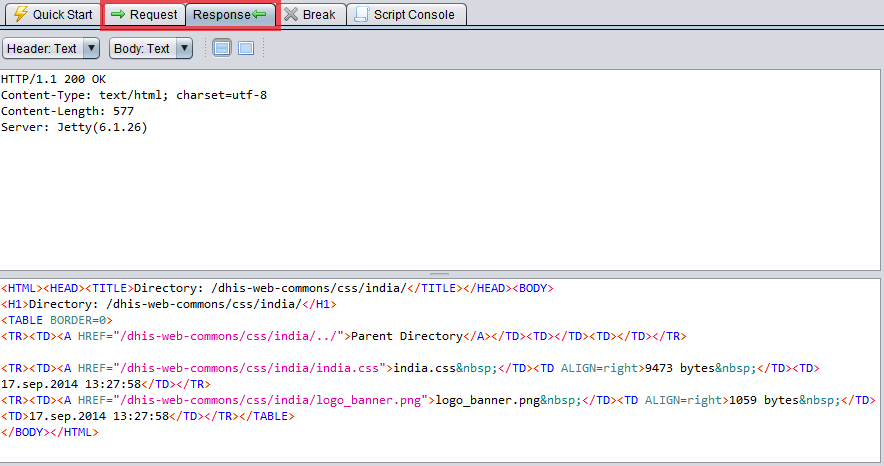
\includegraphics[scale=0.45]{images/zap-right-menu.png}
    \caption{Example of monitoring the network traffic. }
    \label{fig:zaprightmenu}
\end{figure}

\subsubsection{Passive and Active scanner}
The documentation for \gls{zap} states that you should only use \gls{zap} on applications you have permission to do so, as you are actually attacking the application. 
This does not include the passive scanner. 
This is a tool that will run in the background as you browse the application, only listening to the network traffic and not attacking.

\paragraph{}
\gls{zap} also includes an active scanner, which unlike the passive scanner will perform various attacks on the application. 
It is worth noting that the active scanner can only find certain kinds of vulnerabilities. 
So to fully utilize \gls{zap}, you should do manual penetration testing as well as run the active scan.

\begin{figure}[h]
    \centering
    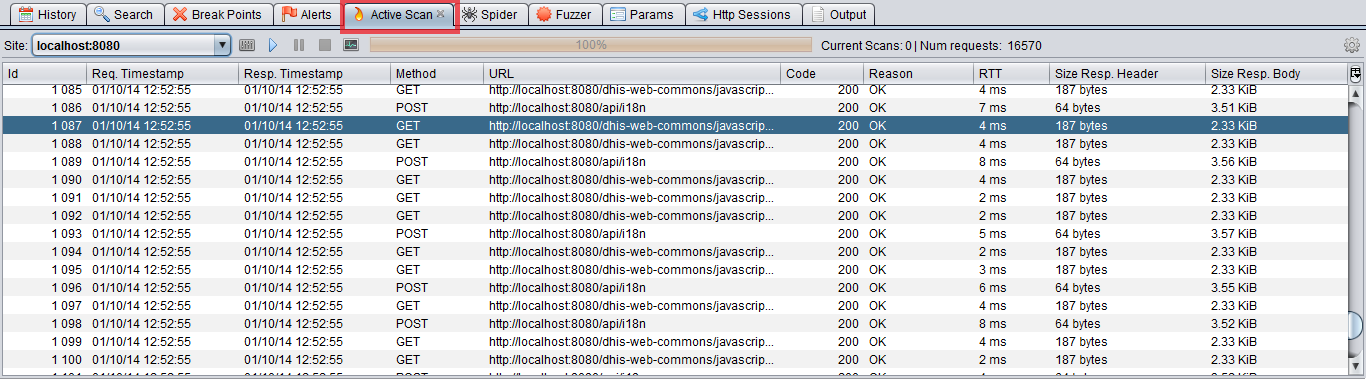
\includegraphics[scale=0.35]{images/zap-active-scan.png}
    \caption{Result of running an active scan. }
    \label{fig:zapactivescan}
\end{figure}

\subsubsection{Spider}
\gls{zap} comes with a built in spider which crawls the application looking for \glspl{url}.
It starts of with the initial list. 
Then it visits all \glspl{url} on the list and finds the \gls{url} resources on each page. 
The spider doesn't stop until it has visited every hyperlink in the application.
The spider will find resources that you may have missed during penetration testing or that has been hidden from you. 
It is a great tool to make sure that you cover the entire application.

\begin{figure}[h]
    \centering
    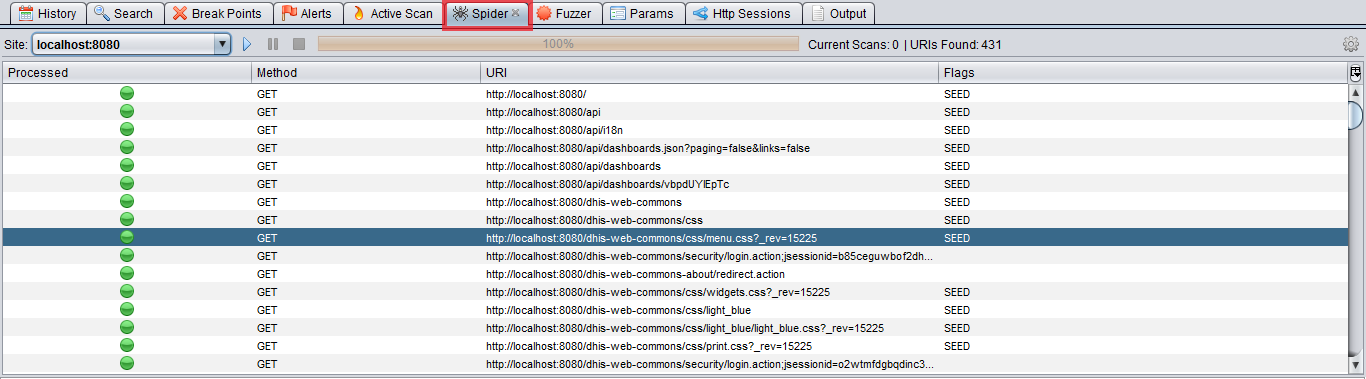
\includegraphics[scale=0.35]{images/zap-spider.png}
    \caption{Result of running the spider. }
    \label{fig:zapspider}
\end{figure}

\subsection{Summary}
\paragraph{}
\gls{zap} is great tool with many helpful features, but that doesn't mean that you can rely solely on the automatic scanners it provides. 
By using \gls{zap} together with manual penetration testing can you achieve the best result and the best coverage. 
Figure~\ref{fig:zapscreenshot}  shows the result of running \gls{zap} on the \gls{dhis} application. You can read more about \gls{zap} here. \cite{zap-documentation,zap-homepage}


\begin{figure}[h]
    \centering
    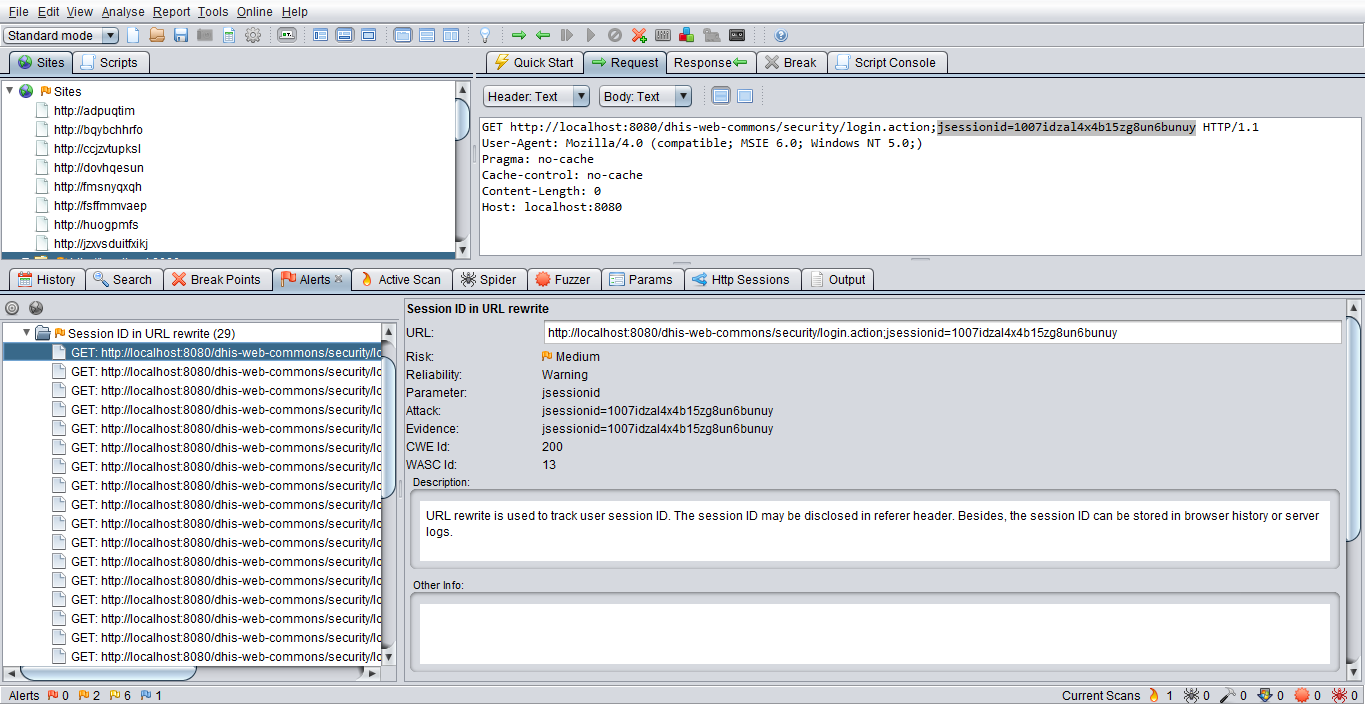
\includegraphics[scale=0.35]{images/zap-sc.png}
    \caption{Screenshot of running \gls{zap} on the codebase}
    \label{fig:zapscreenshot}
\end{figure}


\newpage

\section{HP Fortify}
\paragraph{}
HP Fortify assess, assure and protect enterprise software and applications from security vulnerabilities.
Providing complete security testing and management through static and dynamic testing technologies. 
Or, by repeatable and auditable secure behaviours, over the course of a software application life cycle. 
A flexible delivery model allows security groups to get started quickly and scale in response to business changes while protecting their assets in application security. 
You can read more about HP Fortify here. \cite{fortify-software-wiki, fortify-software-homepage-features} 

\subsection{Installation and Experience}
\paragraph{}
Installing the HP Fortify plug in for Eclipse is a straightforward process. 
First of all, must the HP Fortify software be downloaded and installed.
\gls{uib} provided access to their \gls{svn} repository where the HP Fortify software tool could be downloaded.  
The download includes an installation wizard. 
The default installation covers our needs for this project, however, you can specify specific configurations throughout the wizard. \cite{installation-usage-guide}

\paragraph{}
There exists a HP Fortify plug-in for Eclipse which is easy and convenient to use.
Eclipse has a feature called install new software, where a wizard will take you through the plug-in installation steps.
There you have to specify the installation directory of HP Fortify meaning the HP Fortify software you installed in the previous step.
Here you will have some different configuration settings, for instance what features to install.
After completion of the installation, a simple restart of Eclipse is needed and the menu bar will then include the HP Fortify menu shown in Figure~\ref{fig:fortifymenuscreenshot}. \cite{installation-usage-guide}

\begin{figure}[h]
    \centering
    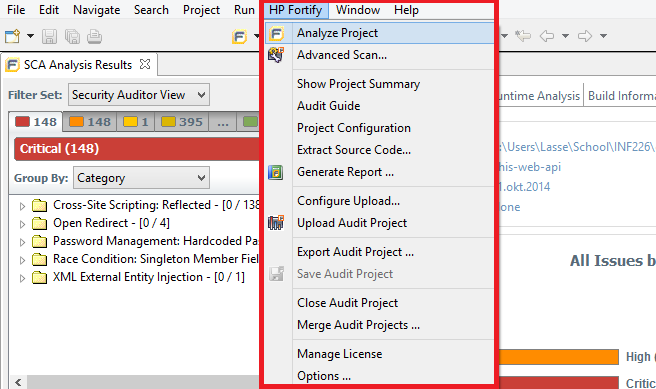
\includegraphics[scale=0.45]{images/fortifymenu-sc.png}
    \caption{After the installation and restart of Eclipse will the HP Fortify menu show in the menu bar of Eclipse.}
    \label{fig:fortifymenuscreenshot}
\end{figure}

\subsection{Features}
\paragraph{}
The plug-in consists of two components: an audit plug-in component and an analysis plug-in component. 
The audit plug-in makes it possible to open and audit former scan results and audit them. 
The analysis plug-in enables you to initiate a \gls{sca} scan and analysis, view the result and fix the discovered security flaws. \cite{installation-usage-guide}

\subsubsection{HP Fortify \gls{sca}}
\paragraph{}
This component makes it possible to initiate a \gls{sca} scan and analysis of your \gls{java} source code.
You can scan entire projects or specify a single package or file that you want to scan. 
Although the plug-in automatically includes all source files from dependencies. 
A scan can easily be started by selecting the desired project, package or file and start the scan from the HP Fortify menu.
The result of the scan will be shown in a new tab in Eclipse, called the \gls{sca} Analysis Result view. \cite{installation-usage-guide}

\paragraph{}
The \gls{sca} Analysis Result view provides a way to group and select security issues that you want to audit. 
Within the view you can set a filter which specifies what issues should be shown, and how they should be listed.
There are many different ways to show the result.
You can for instance choose between Security Auditor View, Developer View, Critical Exposure and Hotspot.

\begin{figure}[h]
    \centering
    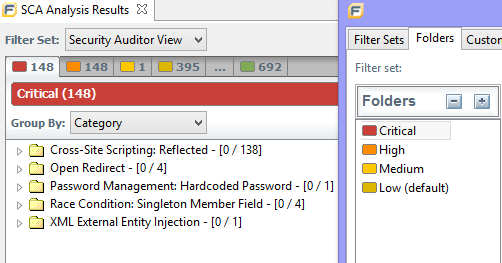
\includegraphics[scale=0.65]{images/fortifyfolders-sc.png}
    \caption{Showing the different color codes for folders. Critical, High, Medium and Low. }
    \label{fig:fortifyfoldersscreenshot}
\end{figure}

\paragraph{}
The issues are sorted by severity, and put into folders accordingly such as critical, high, medium and low. 
When you select an issue, the Analyse Evidence view will be displayed. \cite{installation-usage-guide}

\paragraph{}
\label{analyseevidence}
The Analyse Evidence view presents a justification for why this is an issue.
The view will give a more detailed reason for why this is an issue, and show the direction of the data flow and how the data flow moves. \cite{installation-usage-guide}

\paragraph{}
The Project Summary view displays detailed scan information in different tabs.

\begin{figure}[h]
    \centering
    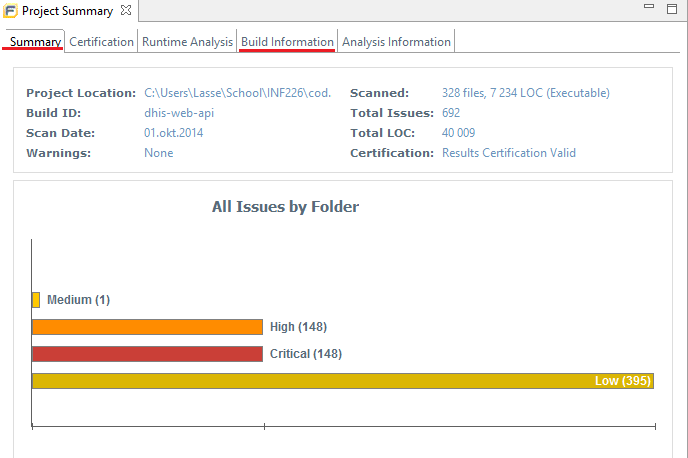
\includegraphics[scale=0.65]{images/fortifysummary-sc.png}
    \caption{Project summary of running a \gls{sca} scan on the codebase. You can switch between different tabs at the top. }
    \label{fig:fortifysummaryscreenshot}
\end{figure}

For instance, a summary tab displaying high-level information about the project and a build information tab showing build id, number of files scanned, date of scan and more applicable information about the scan and project. \cite{installation-usage-guide}

\subsubsection{Auditing Analysis Results}
\paragraph{}
This component is responsible for auditing and analysis of the result.
It is possible to open an existing audit and continue your work.
You can even open the analysis for a project created by someone else on another machine.
If necessary, can you generate a new result from the audit. \cite{installation-usage-guide}

\paragraph{}
The Analysis Evidence view is mentioned in Section~\ref{analyseevidence}. 
It is possible to display the Analyse Evidence view here as well which gives a more detailed reason of a particular issue.
In addition, can you do various of search queries that can contain, be equal/not equal to a text.
You can use \gls{regex} or search for number range and even more. 
Finally can you generate a report based on the analysis data that will show the result of analysis. \cite{installation-usage-guide}


\section{\gls{dhis}}
\paragraph{}
The system is very widespread being the preferred health management information system in 46 countries across five continents. 
The health system helps governments and health organizations to manage their operations more efficiently, monitor processes and improve communication. 
The system is portable and can capture data on any type of device, including desktops, laptops, tablets and smartphones. 
More information about the system can be found here. \cite{dhis2-homepage, dhis2-wiki}

\subsection{Installation and Experience}
\paragraph{}
After following the installation guideline for the codebase found at their homepage, we learned that the information there was insufficient.
It explains how to use \gls{maven} to build the different components and how to set up the database connection, but this only took us so far.
First of all we had to add a new environment variable which specified the location of the database configuration file.
After this, the build was successful, but running the application failed due an OutOfMemoryException. 
This means that the web server didn't have access to enough memory to successfully run the application. 
We fixed this by adding two more environment variables which specified the allocated memory for the \gls{jre} and for \gls{maven}.
Finally the application ran successfully and the project could be built as an Eclipse project and imported into Eclipse where further analysis could be done using HP Fortify.



\chapter{Static Analysis and Penetration Testing Results}
\textit{This chapter will cover the result of running the previously discussed analysis tools on the codebase in an attempt at finding flaws and vulnerabilities.}

\section{\gls{zap}}
\subsection{Approach}
\paragraph{•}
\gls{zap} offers different features which together creates a report which lists the potential issues in the application. 
As discussed in the previous chapter the best approach would be manually using and testing the application relying on intersecting proxy and the passive scanner. 
When this is done the spider and the active scanner can make sure that the entire application is covered as well as doing some automated penetration testing. 
\paragraph{•}
The results will be categorized into security threat level as shown in figure \ref{fig:zapalerts}.
The focus of this report will mostly be on the higher alert levels, but will briefly mention the less important once as well.
The results will be further discussed in section \ref{sec:zapresult}.
\begin{figure}[h]
    \centering
    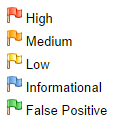
\includegraphics[scale=0.65]{images/alerts.png}
    \caption{Alert levels in \gls{zap}.}
    \label{fig:zapalerts}
\end{figure}
\subsection{Results}
\label{sec:zapresult}
\paragraph{•}
\begin{center}
    \begin{tabular}{| l | l | l | p{5cm} |}
    \hline
    \# & Alert Level & Title & Problem explained \\ \hline
    1 & High
     & 22C & A clear day with lots of sunshine.  
    However, the strong breeze will bring down the temperatures. \\ \hline
    Tuesday & 9C & 19C & Cloudy with rain, across many northern regions. Clear spells
    across most of Scotland and Northern Ireland,
    but rain reaching the far northwest. \\ \hline
    Wednesday & 10C & 21C & Rain will still linger for the morning.
    Conditions will improve by early afternoon and continue
    throughout the evening. \\
    \hline
    \end{tabular}
\end{center}

\section{HP Fortify}
\subsection{Approach}
\subsection{Results}

\chapter{Analysis, Evaluation and Recommendations}

\newpage


\bibliographystyle{plain}
\bibliography{biblio}

\end{document}

